% This text is proprietary.
% It's a part of presentation made by myself.
% It may not used commercial.
% The noncommercial use such as private and study is free
% Sep. 2005 
% Author: Sascha Frank 
% University Freiburg 
% www.informatik.uni-freiburg.de/~frank/
%
% additional usepackage{beamerthemeshadow} is used
%  
%  \beamersetuncovermixins{\opaqueness<1>{25}}{\opaqueness<2->{15}}
%  with this the elements which were coming soon were only hinted
%\documentclass[8pt]{beamer}
\documentclass[10pt]{beamer}
\usepackage{etex}
\newenvironment<>{varblock}[2][\textwidth]{%
  \setlength{\textwidth}{#1}
  \begin{actionenv}#3%
    \def\insertblocktitle{#2}%
    \par%
    \usebeamertemplate{block begin}}
  {\par%
    \usebeamertemplate{block end}%
  \end{actionenv}}
%\usepackage{hyperref}
%\usepackage{natbib}
%\usepackage{beamerthemeshadow}
\usepackage{beamerinnerthemecircles, beamerouterthemeshadow}

\usepackage{amsmath,amssymb,amsfonts}
\usepackage[pdf]{pstricks}
%\usepackage{bbm}
%\usepackage{booktabs}
\usepackage{amsthm}
\usepackage{booktabs}
\usepackage{graphicx}
\usepackage{epsfig}
%\usepackage{graphics}

% MQ: This is to be able to compile on the Riksbank computer. Uncomment with my laptop. Ugly solution but will have to do for now.
%\usepackage{epstopdf}
%\epstopdfsetup{outdir=./}

\usepackage{rotating}

\usepackage{url}
%\usepackage{breqn}
%\usepackage{hyperref}
\usepackage[authoryear]{natbib}
\usepackage{setspace}
\usepackage{multirow}
%\usepackage{harvard}
\usepackage{xcolor}
%\usepackage{multicolumn}
\usepackage{algpseudocode}
\usepackage{sidecap}
\usepackage{bbm} 
\usepackage{courier}
\usepackage{tikz}
\usetikzlibrary{arrows,shapes,snakes,automata,backgrounds,petri}

\tikzset{
  treenode/.style = {align=center, inner sep=0pt, text centered,
    font=\sffamily},
  arn_n/.style = {treenode, circle, white, font=\sffamily\bfseries, draw=black,
    fill=black, text width=1.5em},% arbre rouge noir, noeud noir
  arn_r/.style = {treenode, circle, red, draw=red, 
    text width=1.5em, very thick},% arbre rouge noir, noeud rouge
  arn_x/.style = {treenode, rectangle, draw=black,
    minimum width=0.5em, minimum height=0.5em}% arbre rouge noir, nil
}
\beamertemplatenavigationsymbolsempty

\newenvironment{myenumerate}{\begin{enumerate}[(1)]}{\end{enumerate}} 
\sidecaptionvpos{figure}{c}
% FOR COLORING PARTS  OF TABLE
%\usepackage[beamer,customcolors]{hf-tikz}

%\tikzset{hl/.style={
%    set fill color=red!80!black!40,
%    set border color=red!80!black,
%  },
%}

\mode<presentation> {
    \usetheme{Madrid} %Frankfurt} %Bergen, Berkely, Berlin, Boadilla, CambridgeUS, Darmstadt,
                          %Frankfurt, Goettingen, Singapore, Warsaw
    \usecolortheme{beaver} %seahorse} %default} %beetle, seahorse, wolverine, dolphin, beaver
    %\useoutertheme[subsection=true]{smoothbars} 
    \usefonttheme{default}
    %\usecolortheme{red}
    

	\setbeamercolor{block title}{use=unstructure, fg=white, bg=purple!75!black} %{use=structure,fg=white,bg=purple!75!black}
	%\setbeamercolor{block body}{use=structure,fg=black,bg=white!20!white}    
    %\setbeamercolor{block body}{bg=white}
    \setbeamertemplate{enumerate items}[default]
    \setbeamercolor{enumerate item}{fg=purple!75!black} 
    \setbeamercolor{enumerate subitem}{fg=purple!75!black} 	 
	\setbeamercolor{itemize item}{fg=purple!75!black}  
	\setbeamertemplate{itemize item}[triangle]  
	\setbeamercolor{itemize subitem}{fg=purple!75!black}
	\setbeamertemplate{itemize subitem}[triangle]
	\setbeamertemplate{blocks}[framed]


}



%\usepackage{colortbl}
%\definecolor{yellow}{cmyk}{0,0.18,0.90,0.00}

%\usepackage{xcolor}

%\usepackage[authoryear]{natbib}
\begin{document}
\title[Lecture 4]{Bayesian Learning 732A46: Lecture 4}  
\author[Matias Quiroz]{Matias Quiroz\inst{1}$^{,}$\inst{2}}
\setbeamerfont{institute}{size=\fontsize{7pt}{8pt}}
\institute[LiU and Riksbank]{
  \inst{1}%
   Division of Statistics and Machine Learning, Link\"{o}ping University\\~\\
  \inst{2}%
   Research Division, Sveriges Riksbank\\
     
}

%\institute[Riksbank and LiU]{Sveriges Riksbank and Division of Statistics and Machine Learning, Link\"{o}ping University}

\date[]{April 2016} %\today 

%\usebackgroundtemplate{%
%  \vbox to \paperheight{\vfil\hbox to \paperwidth{\hfil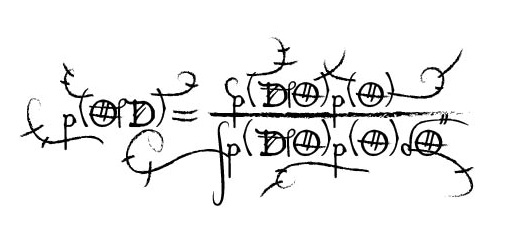
\includegraphics[width=1.5in]{Bayes.jpg}\hfil}\vfil}
%}

{
%\usebackgroundtemplate{\begin{center}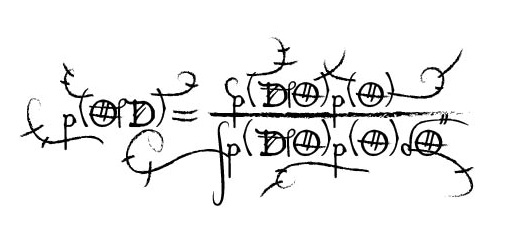
\includegraphics[width=0.4\paperwidth]{Bayes.jpg}\end{center}}
\usebackgroundtemplate{%
  \vbox to \paperheight{\hbox to \paperwidth{\hfil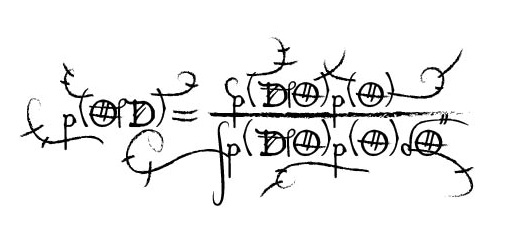
\includegraphics[width=2in]{Bayes.jpg}\hfil}}
}
\begin{frame}
\titlepage
\end{frame}
}
%\frame{\titlepage} 

%\frame{\frametitle{Overview of the talk}\tableofcontents}

\begin{frame}{Lecture overview}

\begin{itemize}
\item \textbf{\textcolor{blue}{Prediction}}

\begin{itemize}
\item Normal model
\item Complex predictions by simulation
\end{itemize}
\item \textbf{\textcolor{blue}{Decision theory}}

\begin{itemize}
\item The elements of a decision problem
\item The Bayesian way
\item Point estimation as a decision problem
\end{itemize}
\end{itemize}
\end{frame}

\begin{frame}{Prediction/Forecasting}

\begin{itemize}
\item \textbf{\textcolor{blue}{Posterior predictive distribution}} for future
$\tilde{y}$ given observed data $y$
\[
p(\tilde{y}|y)=\int_{\theta} p(\tilde{y},\theta | y)d\theta = \int_{\theta}p(\tilde{y}|\theta,y)p(\theta|y)d\theta.
\]
\bigskip{}

\item \textbf{\color{blue}Note}: Averages $p(\tilde{y}|\theta, y)$ over the posterior distribution $p(\theta|y)$ $\implies$ predictions \textbf{take into account the parameter uncertainty}.
\bigskip{}

\item \textbf{\color{blue}Simplified} if $p(\tilde{y}|\theta,y)=p(\tilde{y}|\theta)$ {[}not true for time
series{]}, then 
\[
p(\tilde{y}|y)=\int_{\theta}p(\tilde{y}|\theta)p(\theta|y)d\theta.
\]
\item \textbf{\color{red}Easy} to simulate (marginalization by simulation)
\begin{eqnarray*}
\theta^{(i)} & \sim & p(\theta|y) \\
\tilde{y}^{(i)} | \theta^{(i)} & \sim & p(\tilde{y}|\theta^{(i)})
\end{eqnarray*}
\item \textbf{Histogram} (or \textbf{Kernel density estimate}) of $\tilde{y}^{(i)}$ is an approximation of $p(\tilde{y} |y)$.

\end{itemize}
\end{frame}

\begin{frame}{Prediction - Normal data, known variance}

\begin{itemize}
\item Our old friend $$y_i | \theta \overset{iid}{\sim} \mathcal{N}(\theta,\sigma^{2})\quad [\textbf{\color{red}known } \sigma^2 ]$$
\item The \textbf{\color{blue}posterior predictive}
\[
p(\tilde{y}|y)=\int_{\theta}p(\tilde{y}|\theta)p(\theta|y)d\theta,
\]
where, if  $p(\theta) \propto c$ (\textbf{uniform} prior), 
\begin{eqnarray*}
\theta|y & \sim & \mathcal{N}(\bar{y},\sigma^{2}/n)\\
\tilde{y}|\theta & \sim & \mathcal{N}(\theta,\sigma^{2})
\end{eqnarray*}

\end{itemize}

%\pause{}
\begin{enumerate}
\item Generate a posterior draw of $\theta$ [$\theta^{(1)}$] from $\mathcal{N}(\bar{y},\sigma^{2}/n)$
\item Generate a draw of $\tilde{y}$ [$\tilde{y}^{(1)}$] from $\mathcal{N}(\theta^{(1)},\sigma^{2})$
({\color{blue}note the mean})
\item \textbf{Repeat} Steps 1 and 2 a large number of times ($N$) with the result:

\begin{itemize}
\item {\color{blue}Sequence of posterior draws}: $\ \theta^{(1)},....,\theta^{(N)}$
\item {\color{blue}Sequence of predictive draws}: $\tilde{y}^{(1)},...,\tilde{y}^{(N)}$. 
\end{itemize}
\end{enumerate}
\end{frame}

\begin{frame}{Predictive distribution - Normal model and uniform prior}

\begin{itemize}
\item In this simple model it is\textbf{ easy to derive} $p(\tilde{y}|y)$ analytically.
\item Note that 
\begin{enumerate}
\vspace{2mm}
\item[Step 1.] $\theta^{(i)} = \bar{y} + \omega^{(i)}, \quad \omega^{(i)} \sim \mathcal{N}(0, \sigma^2/n)$
\vspace{2mm}
\item[Step 2.] $\tilde{y}^{(i)} = \theta^{(i)} + \varepsilon^{(i)}, \quad \varepsilon^{(i)} \sim \mathcal{N}(0, \sigma^2)$
\end{enumerate}
\item $\varepsilon^{(i)}$ and $\upsilon^{(i)}$ are independent.
\item The sum of two normal r.v's is normal so $p(\tilde{y}|y)$ is normal, 
\begin{eqnarray*}
E(\tilde{y}|y) & = & \bar{y}\\
V(\tilde{y}|y) & = & \frac{\sigma^{2}}{n}+\sigma^{2}=\sigma^{2}\left(1+\frac{1}{n}\right)
\end{eqnarray*}
\[
\tilde{y}\vert y\sim \mathcal{N}\left(\bar{y},\sigma^{2}\left(1+\frac{1}{n}\right)\right).
\]

\end{itemize}
\end{frame}

\begin{frame}{Predictive distribution - Normal model and normal prior}
\begin{itemize}
\item Assume still that $\sigma^2$ \textbf{is known}, but
$$p(\theta) = \mathcal{N}(\theta | \mu_0, \tau^2_0) \implies p(\theta|y)=\mathcal{N}(\theta | \mu_n, \tau^2_n)$$
\vspace{-5mm}
\begin{enumerate}
\vspace{2mm}
\item[Step 1.] $\theta^{(i)} = \mu_n + \omega^{(i)}, \quad \omega^{(i)} \sim \mathcal{N}(0, \tau_n^2)$
\vspace{2mm}
\item[Step 2.] $\tilde{y}^{(i)} = \theta^{(i)} + \varepsilon^{(i)}, \quad \varepsilon^{(i)} \sim \mathcal{N}(0, \sigma^2)$
\end{enumerate}
\vspace{2mm}
with (which \textbf{you know} by \textbf{{\color{red}heart}} now!)
$$\frac{1}{\tau^2_n}=\frac{1}{\tau^2_0} + \frac{n}{\sigma^2}\quad	\text{and} \quad \mu_n = \left(\frac{1}{\tau^2_0} \mu_0 +   \frac{n}{\sigma^2}\bar{y} \right)\bigg/\frac{1}{\tau^2_n}.$$
\item It easy to see that the \textbf{predictive distribution} is normal. 
\item \textbf{With mean} [\textbf{\color{blue}Tower Property} or \textbf{\color{blue}Law of total (conditional) expectation}]
$$E\left(\tilde{y}|y\right) =E_{\theta|y}\left(E_{\tilde{y}|\theta, y}\left(\tilde{y}|\theta, y\right) \right)= E_{\theta|y}\left(\underbrace{E_{\tilde{y}|\theta}\left(\tilde{y}|\theta\right)}_{\theta} \right) = \mu_n $$
\item \text{Note that} $\tilde{y}$ and $y$ are \textbf{\color{blue}conditionally independent given} $\theta$.

\end{itemize}
\end{frame}


\begin{frame}{Predictive distribution - Normal model and normal prior, cont}
\begin{itemize}

\item \textbf{And variance} [\textbf{\color{blue}Law of total (conditional) variance} + $p(\tilde{y}|\theta,y )= p(\tilde{y}|\theta)$]
\begin{eqnarray*}
V(\tilde{y}|y) & = & E_{\theta|y}[V_{\tilde{y}|\theta}(\tilde{y}|\theta)]+V_{\theta|y}[E_{\tilde{y}|\theta}(\tilde{y}|\theta)]\\
 & = & E_{\theta|y}(\sigma^{2})+V_{\theta|y}(\theta)\\
 & = & \sigma^{2}+\tau_{n}^{2}\text{ \ }\\
 & = & \text{(\textbf{{\color{red}Population variance} + {\color{red}Posterior variance}} of }\theta\text{).}
\end{eqnarray*}

\item In \textbf{\textcolor{blue}{summary}}: 
\[
\tilde{y}|y\sim \mathcal{N}(\mu_{n},\sigma^{2}+\tau_{n}^{2}).
\]

\end{itemize}
\end{frame}

\begin{frame}{Bayesian prediction in a more complex model}

\begin{itemize}
\item \textbf{\textcolor{blue}{Autoregressive process}}
\begin{eqnarray*}
y_{t} & = & \phi_{1}(y_{t-1}-\mu)+...+\phi_{p}(y_{t-p}-\mu)+\varepsilon_{t},\text{ \ensuremath{\varepsilon_{t}\overset{iid}{\sim}\mathcal{N}(0,\sigma^{2})}}
\end{eqnarray*}
\item Note that $\tilde{y}$ and $y$ are \textbf{\color{red}not conditionally independent given} $\theta$
\item \textbf{Why not}? 
\begin{itemize}
\item \textbf{Conditional independence} means that \textbf{\color{blue}if I know} $\theta$, I can simulate $$\tilde{y} \sim p(\tilde{y}|\theta,y)=p(\tilde{y}|\theta),$$i.e. \textbf{\color{blue}without caring} about $y$.
\item Let $p=1$ and suppose we want $\tilde{y}_{T+1}$. Let $\theta=(\phi_{1},\mu,\sigma)$ be given, then
$$\tilde{y}_{T+1}  =  \phi_{1}(y_{T}-\mu) + \varepsilon_{T}, \quad \varepsilon_{T}\sim \mathcal{N}(0,\sigma^{2})$$
\item We need $y_T \subset y$. \textbf{They can't be independent, even if we know $\theta$}!
\end{itemize}

\item \textbf{No worries}, we can still do predictions (slightly more to keep in mind).



\end{itemize}
\end{frame}


\begin{frame}{Bayesian prediction in a more complex model, cont.}

\begin{itemize}
\item \textbf{\textcolor{blue}{Autoregressive process}}
\begin{eqnarray*}
y_{t} & = & \phi_{1}(y_{t-1}-\mu)+...+\phi_{p}(y_{t-p}-\mu)+\varepsilon_{t},\text{ \ensuremath{\varepsilon_{t}\overset{iid}{\sim}\mathcal{N}(0,\sigma^{2})}}
\end{eqnarray*}

\item $K$-step ahead prediction of $\tilde{y}$  - \textbf{\color{red}"roll simulation forward $K$-steps"}.
\item \textbf{\color{blue}Simulate} a draw from $p(\phi_{1},\phi_{2},...,\phi_{p},\mu,\sigma|y)$

\begin{itemize}
\item Conditional on that draw $\theta^{(1)}=(\phi_{1}^{(1)},\phi_{2}^{(1)},...,\phi_{p}^{(1)},\mu^{(1)},\sigma^{(1)})$,
simulate 
\medskip
\item $\tilde{y}_{T+1}\sim$ $p(y_{T+1}|y_{T},y_{T-1},...,y_{T+1-p},\theta^{(1)})$
\medskip
\item $\tilde{y}_{T+2}\sim p(y_{T+2}|\tilde{y}_{T+1},y_{T},...,y_{T+2-p},\theta^{(1)})$
\item[] $\vdots$
\item $\tilde{y}_{T+K}\sim p(y_{T+K}|\tilde{y}_{T+K-1},\tilde{y}_{T+K-2},...,y_{T+K-p},\theta^{(1)})$ [if $K\leq p$, otherwise $\sim$] % $\tilde{y}_{T+ K-p}$ ]
\end{itemize}
\item \textbf{\color{blue}Repeat} for new $\theta$ draws.
\end{itemize}

\end{frame}

\begin{frame}{Decision Theory}

\begin{itemize}
\item \textbf{Brief} introduction. See the \textbf{\color{blue}excellent} Berger (2013) book.
\item Let $\theta \in \Theta$ be an \textbf{\textcolor{blue}{unknown quantity}}. \textbf{\textcolor{blue}{State
of nature}}. \\ \textbf{Examples}: \textit{Future inflation, Global temperature, Disease}.
\item Let $a\in\mathcal{A}$ be an \textbf{\textcolor{blue}{action}}.  \textbf{Examples}:
\textit{Interest rate, Energy tax, Surgery}.
\item \textbf{Choosing action} $a$ (=decision) when state of nature turns out to be $\theta$
gives \textbf{\textcolor{blue}{utility}}
\[
U(a,\theta)
\]
\vspace{-5mm}
\item Alternatively \textbf{\textcolor{blue}{loss}} $L(a,\theta)=-U(a,\theta)$.\bigskip{}
\vspace{-3mm}
\small{
\item \textbf{Loss table}:\hspace{2cm} %
\begin{tabular}{c|cc}
 & $\theta_{1}$ & $\theta_{2}$\tabularnewline
\hline 
$a_{1}$ & $L(a_{1},\theta_{1}$) & $L(a_{1},\theta_{2}$)\tabularnewline
$a_{2}$ & $L(a_{2},\theta_{1}$) & $L(a_{2},\theta_{2}$)\tabularnewline
\end{tabular}
\item \textbf{Example}:\hspace{2cm} %
\begin{tabular}{c|cc}
 & Rainy & Sunny\tabularnewline
\hline 
Umbrella & 20 & 10\tabularnewline
No umbrella & 50 & 0\tabularnewline
\end{tabular}}
\item \textbf{The decision problem}: Choose \textbf{an action} $a$ that \textbf{minimizes the loss}.
%\item ... but the loss is \textbf{stochastic} (\textbf{\color{blue}Frequentist}: data, \textbf{\color{blue}Bayesian}: parameter)
\end{itemize}

\end{frame}

\begin{frame}{Decision Theory, cont.}

\begin{itemize}
\item Example \textbf{\textcolor{blue}{loss functions}} when both $a$ and
$\theta$ are continuous: 

\begin{itemize}
\item \textcolor{blue}{Linear}: $L(a,\theta)=\left|a-\theta\right|$
\item \textcolor{blue}{Quadratic}: $L(a,\theta)=(a-\theta)^{2}$
\item \textcolor{blue}{Lin-Lin}: 
\[
L(a,\theta)=\begin{cases}
c_{1}\cdot\left|a-\theta\right| & \textrm{if \ensuremath{a\leq\theta}}\\
c_{2}\cdot\left|a-\theta\right| & \textrm{if \ensuremath{a>\theta}}
\end{cases}
\]

\end{itemize}
\item \textbf{\color{blue}Example}: 

\begin{itemize}
\item $\theta$ is the \textbf{number of items} demanded of a product
\item $a$ is the \textbf{number of items} in stock
\item Loss

\[
L(a,\theta)=\begin{cases}
10 \cdot (\theta-a) & \textrm{if \ensuremath{a\leq\theta}\text{ [too little stock]}} \\
~~1 \cdot (a-\theta) & \textrm{if \ensuremath{a>\theta}\text{ [too much stock]}}\\
\end{cases}.
\]

\item We are \textbf{punished} by a factor of 10 for keeping \textbf{too little} in stock.


%\[
%U(a,\theta)=\begin{cases}
%p\cdot\theta-c_{1}(a-\theta) & \textrm{if \ensuremath{a>\theta}\text{ [too much stock]}}\\
%p\cdot a-c_{2}(\theta-a)^{2} & \textrm{if \ensuremath{a\leq\theta}\text{ [too little stock]}}
%\end{cases}
%\]

\end{itemize}
\end{itemize}
\end{frame}

\begin{frame}{Optimal decision}

\begin{itemize}
%\item Ad hoc decision rules:

%\begin{itemize}
%\item \emph{Minimax}. Choose the decision that minimizes the maximum loss. 
%\item \emph{Minimax-regret} ... bla bla bla ...
%\end{itemize}
\item Bayesian choice: maximize the \textbf{\textcolor{blue}{posterior
expected utility}}:
\[
a_{bayes}=\mathrm{argmax}{}_{a\in\mathcal{A}}\text{ }E_{\theta|y}\left(U(a,\theta)\right),
\]
where $E_{\theta|y}$ denotes the \textbf{posterior expectation,}
$$E_{\theta|y}\left(U(a,\theta)\right) = \int_{\theta \in \Theta}  U(a,\theta) p(\theta|y) d\theta $$
\medskip
\item \textbf{\color{blue}Easy} to estimate by simulation (\textbf{\color{blue}LLN}): 
\[
\text{ }E_{\theta|y}\left(U(a,\theta)\right)\approx \frac{1}{N}\sum_{i=1}^{N}U(a,\theta^{(i)}) \quad  \theta^{(i)} \sim p(\theta| y)
\]
\medskip
\item \textbf{\color{blue}Note}: we could have \textbf{\color{red}minimized} the \textbf{\textcolor{blue}{posterior expected {\color{red}loss}}} .

\end{itemize}


\end{frame}




\begin{frame}{Choosing a point estimate is a decision}

\begin{itemize}
\item Choosing a \textbf{\textcolor{blue}{point estimator}} is a decision
problem. 
\medskip
\item Possible  \textbf{\color{blue}action space}
$$\mathcal{A} = \{\theta_{\mathrm{median}}, \theta_{\mathrm{mode}}, \theta_{\mathrm{mean}} \}.$$
\end{itemize}

\medskip{}

\begin{itemize}
\item Which one is the \textbf{optimal choice}?
\end{itemize}

\medskip{}

\begin{itemize}
\item \textbf{It depends on the loss function}:

\begin{itemize}
\item \textbf{\color{blue}Linear loss }$\rightarrow$ \textbf{Posterior median} is optimal
\vspace{0.5mm}
\item \textbf{\color{blue}Quadratic loss }$\rightarrow$ \textbf{Posterior mean} is optimal
\vspace{0.5mm}
\item \textbf{\color{blue}Lin-Lin loss }$\rightarrow$ $c_{2}/(c_{1}+c_{2})$ \textbf{ posterior quantile} is optimal
\vspace{0.5mm}
\item \textbf{\color{blue}Zero-one loss} $\rightarrow$ \textbf{Posterior mode} is optimal
\end{itemize}
\end{itemize}

\medskip{}
\end{frame}

\begin{frame}
\frametitle{References}

\small{
\textbf{Berger, J. (2013)}.  \textit{Statistical decision theory and Bayesian analysis}. Springer Science \& Business Media.}


\end{frame}

\end{document}

